\let\negmedspace\undefined
\let\negthickspace\undefined
\documentclass[journal,12pt,twocolumn]{IEEEtran}
\usepackage{cite}
\usepackage{amsmath,amssymb,amsfonts,amsthm}
\usepackage{algorithmic}
\usepackage{graphicx}
\usepackage{textcomp}
\usepackage{xcolor}
\usepackage{txfonts}
\usepackage{listings}
\usepackage{enumitem}
\usepackage{mathtools}
\usepackage{gensymb}
\usepackage{comment}
\usepackage[breaklinks=true]{hyperref}
\usepackage{tkz-euclide} 
\usepackage{listings}                                     
\def\inputGnumericTable{}                                 
\usepackage[latin1]{inputenc}                                
\usepackage{color}                                            
\usepackage{array}                                            
\usepackage{longtable}                                       
\usepackage{calc}                                             
\usepackage{multirow}                                         
\usepackage{hhline}                                           
\usepackage{ifthen}                                           
\usepackage{lscape}

\newtheorem{theorem}{Theorem}[section]
\newtheorem{problem}{Problem}
\newtheorem{proposition}{Proposition}[section]
\newtheorem{lemma}{Lemma}[section]
\newtheorem{corollary}[theorem]{Corollary}
\newtheorem{example}{Example}[section]
\newtheorem{definition}[problem]{Definition}
\newcommand{\BEQA}{\begin{eqnarray}}
\newcommand{\EEQA}{\end{eqnarray}}
\newcommand{\define}{\stackrel{\triangle}{=}}
\theoremstyle{remark}
\newtheorem{rem}{Remark}
\begin{document}

\bibliographystyle{IEEEtran}
\vspace{3cm}

\title{NCERT 12.8 Q4}
\author{EE23BTECH11014 - Devarakonda Guna Vaishnavi $^{}$% <-this % stops a space
}
\maketitle
\newpage
\bigskip

\renewcommand{\thefigure}{\theenumi}
\renewcommand{\thetable}{\theenumi}

\bibliographystyle{IEEEtran}


\textbf{Question:} A plane electromagnetic wave travels in vacuum along the \(z\)-direction. What can you say about the directions of its electric (\(\mathbf{E}\)) and magnetic (\(\mathbf{B}\)) field vectors? If the frequency of the wave is \(30 \, \text{MHz}\), what can you say about its wavelength?
 

\textbf{Solution:} 
\begin{table}[h]
    \centering
    

\begin{tabular}{|c|l|c|}
\hline
Symbol & Description                               & Value                    \\ \hline
\(c\)    & Speed of light in vacuum                  & \(3 \times 10^8 \, \text{m/s}\) \\
\(f\)    & Frequency of the electromagnetic wave    & \(30 \, \text{MHz}\)     \\
\(\lambda\) & Wavelength of the electromagnetic wave   & ?                        \\ \hline
\end{tabular}


    \caption{Input Parameters}
    \label{table:parameters}
\end{table}

\begin{figure}[h!]
	\centering
	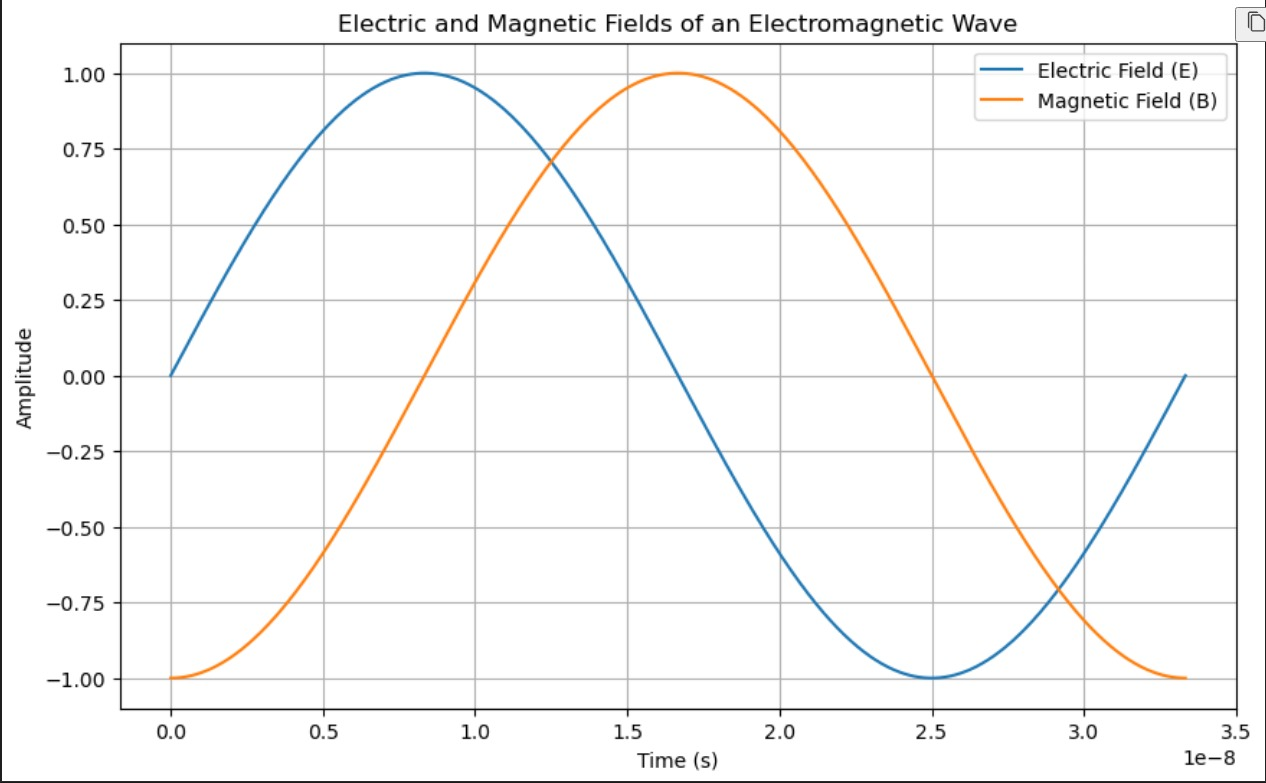
\includegraphics[width=\columnwidth]{emfigs/emplot.jpeg}
	\label{fig:plot}
\end{figure}

\textbf{} 
 a) A plane electromagnetic wave travels in vacuum along the \(z\)-direction. The electric (\(\mathbf{E}\)) and magnetic (\(\mathbf{B}\)) field vectors are perpendicular to each other move in x and y direction respectively and they are perpendicular to each other
 \vspace{0.2cm}

 b)The relationship between frequency (\(f\)), wavelength (\(\lambda\)), and the speed of light (\(c\)) is given by the formula:
\begin{align}
        \lambda = \frac{c}{f}
    \end{align}


\begin{align}
        \lambda &= \frac{3 \times 10^8 \, \text{m/s}}{30 \times 10^6 \, \text{Hz}} \\
        &= 10 \, \text{m}
    \end{align}
    
$\implies \lambda = 10m$




\end{document}
